Testing the fully assembled robot was conducted in two analogous but distinct phases, one for each configuration of AFER. Phase 1 tested the performance of AFER v1, and Phase 2 involved the same testing for AFER v2. The testing questions answered for both versions are listed below:
\begin{itemize}
\item Is the base adequately secured?
\item Does the up/down oscillation function under load?
\item Does the left/right oscillation function under load?
\item Does the combined oscillation function under load?
\item Do the chosen trajectories avoid self-collision?
\item Are the wires adequately concealed?
\item Have all obstacles been removed from the area?
\item Is the end effector securely attached?
\end{itemize}

Results for all tests were collected using visual observation, and servo outputs. Visual observation was the primary method of ascertaining proper behavior of the system, however the servo output data was also analyzed in real time to verify proper operation of the robot. Once the robot was determined to be operational and safe, the test subjects were introduced. 
The following procedure was used to ascertain the test subject’s interaction preferences between AFER v1 and AFER v2 robots and the type of end effector. Those steps were recorded and evaluated based on visual observation: 
\begin{itemize}
\item Introduce test subjects (cats) to base configuration
\item Assemble AFER v1
\item Introduce test subjects to v1 configuration
\item Allow test subjects to interact with operational AFER v1 with End Effector 1 attached
\item Allow test subjects to interact with operational AFER v1 with End Effector 2 attached
\item Observe and record test subject behavior
\item Repeat steps 2-6 with the AFER v2 configuration
\end{itemize}

Fig. 7 shows the engagement of kittens with AFER v1 and v2. Basic standards for ethical treatment of animals were obeyed when observing the cats/kittens engaged with the robots \cite{Brambell1965ReportOT}.

\begin{figure}[h!]
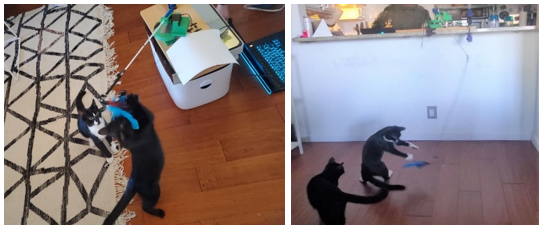
\includegraphics[width=\columnwidth]{Fig7.png}
\caption{Kittens engaged with AFER v1 (left) and v2 (right).}
\end{figure}

